\documentclass{oci}
\usepackage[utf8]{inputenc}
\usepackage{lipsum}

\title{Transbordo en el aeropuerto}

\begin{document}
\begin{problemDescription}
  A Lucas le encanta viajar.
  Lo hace varias veces al año, escogiendo siempre un nuevo destino para conocer.
  Para ahorrar dinero, y así poder viajar más, Lucas siempre toma los vuelos más
  baratos.
  Esto suele ser un problema pues a menudo tiene que realizar escalas y correr
  para alcanzar el siguiente avión.

  Los aeropuertos están siempre divididos en \emph{terminales}.
  Cuando Lucas se baja de un avión lo hace en un terminal de inicio $S$ y luego
  tiene que recorrer el aeropuerto hasta llegar a un terminal de destino
  $T$.
  Los terminales dentro de un aeropuerto están conectados por caminos que Lucas
  puede atravesar caminando en ambos sentidos.
  Después de tantos viajes Lucas ya conoce prácticamente todos los aeropuertos
  y tiene un mapa de cada uno de estos con los caminos que hay entre terminales
  junto con el tiempo que tarda en recorrerlos.

  Muchas veces es imposible recorrer los aeropuertos solo caminando así que
  estos ponen a disposición trenes entre algunos terminales.
  Lucas también ha recolectado la información de estos trenes y tiene un
  itinerario de viajes con el momento exacto en que los trenes partirán de cada
  terminal y el tiempo que tardarán en llegar al terminal de destino.

  La figura de más abajo muestra un aeropuerto de ejemplo con tres terminales.
  Las lineas continuas representan los caminos que Lucas puede atravesar
  caminando y las líneas punteadas los trayectos en tren.
  El número junto a los caminos representa el tiempo en minutos que Lucas tarda
  en recorrerlos.
  El primer número junto a los trayectos en tren representa el momento en que
  el recorrido partirá del terminal medido como la cantidad de minutos desde
  que Lucas inicia su recorrido.
  El segundo número corresponde al tiempo en minutos que el tren tardará en
  llegar a su destino.
  Por ejemplo, justo en el momento que Lucas inicia su recorrido un tren saldrá
  desde el terminal 3 hacia el 1 y demorará 5 minutos en llegar a su destino.
  Después de 3 minutos, un tren desde el terminal 2 hacia el 3 comenzará su
  trayecto tardando 6 minutos.
  Posteriormente, luego de tres minutos desde la partida de este tren (6 minutos
  desde que Lucas comenzó), un tren entre los mismos terminales iniciará su
  trayecto y tardará 7 minutos.
  Finalmente, 30 minutos después de que Lucas comience su recorrido partirá un
  tres desde el terminal 1 al 3 y tardará 5 minutos.

  \begin{center}
  \includegraphics[scale=0.7]{aeropuerto}
  \end{center}

  Si Lucas debe partir desde el terminal 1 y llegar al 3 tiene varias
  alternativas.
  La primera es esperar 30 minutos a que el tren parta desde el terminal 1 hacia
  el 3.
  Estos 30 minutos de espera más los 5 minutos que tarda el tren dan un total de
  35 minutos para el recorrido total.
  Otra alternativa es caminar hacia el terminal 2 tardando 5 minutos.
  En este momento Lucas ya perdió la posibilidad de tomar el primer tren que
  parte de está estación, pero puede esperar un minuto y tomar el segundo tren.
  Contando los 7 minutos que este tarda en llegar a su destino da un total de 13
  minutos para llegar del terminal 1 al 3.
  La última alternativa es caminar por 20 minutos entre el terminal 2 y 3
  tardando un total de 25 minutos en todo el recorrido.
  Por lo tanto, en el mejor caso Lucas tarda 13 minutos en llegar a su destino.

  Dada la descripción de un aeropuerto, un terminal de inicio $S$ y uno de
  destino $T$, a Lucas le gustaría saber el menor tiempo en que es posible
  trasladarse desde $S$ a $T$.
  Lucas ya está cansado de perder vuelos.
  ?`Podrías ayudarlo?
\end{problemDescription}

\begin{inputDescription}
  La primera línea de la entrada contiene cuatro enteros $N$, $M$, $S$ y $T$
  ($0 < N\leq 1000, 0 < M \leq 10000$, $1 \leq S, T\leq N$).
  Los enteros $N$ y $M$ corresponden respectivamente a la cantidad de terminales
  y de caminos en el aeropuerto.
  Cada terminal es identificado con un número entre 1 y $N$.
  Los enteros $S$ y $T$ corresponden respectivamente al terminal de inicio y de
  destino.

  Posteriormente cada una de las siguientes $M$ líneas contienen tres enteros
  $a$, $b$ y $c$ ($1\leq a, b\leq N$ y $0<c\leq 1000$) indicando que existe un
  camino entre el terminal $a$ y el terminal $b$ y que Lucas tarda $c$ minutos
  en recorrerlo.
  Se garantiza que siempre será posible moverse entre cualquier par de
  terminales usando solamente estos caminos.

  A continuación sigue una línea con un entero $P$ correspondiente a la
  cantidad de entradas que contiene el itinerario de viajes en tren.
  Cada una de las siguientes $P$ líneas contiene cuatro enteros $u$, $v$,
  $t$ y $w$ ($1 \leq u,v \leq N, 0\leq t\leq 10^9, 0 < w \leq 1000$)
  describiendo un trayecto en tren. 
  Los enteros indican que el tren viajará desde el terminal $u$ hasta el
  terminal $v$, que partirá $t$ minutos después de que Lucas comienza su
  recorrido y que este se demorará $w$ minutos en llegar al destino.
\end{inputDescription}

\begin{outputDescription}
  La salida debe contener un solo entero correspondiente al tiempo mínimo en que
  Lucas puede llegar desde $S$ a $T$.
\end{outputDescription}

\begin{scoreDescription}
  \score{5} Se probarán varios casos en que no hay trayectos en tren ($P=0$) y
  los terminales junto a los caminos formarán una línea, es decir, el primer
  terminal está conectado al segundo, el segundo con el tercero, etc (ver
  el primer ejemplo de entrada). 
  \score{10} Se probarán varios casos en que los terminales junto a los caminos
  forman una línea como en la subtarea anterior, pero además es posible que haya
  un trayecto en tren entre terminales consecutivos, es decir, puede haber un
  tren entre el terminal $i$ y el $i+1$ o entre el $i+1$ y el $i$ (ver segundo
  ejemplo de entrada).
  \score{35} Se probarán varios casos sin trayectos en tren ($P=0$) y sin
  restricciones en los caminos (ver tercer ejemplo de entrada).
  \score{50} Se probarán varios casos sin restricciones adicionales (ver cuarto
  ejemplo de entrada).
\end{scoreDescription}

\begin{sampleDescription}
\sampleIO{sample-1}
\sampleIO{sample-2}
\sampleIO{sample-3}
\sampleIO{sample-4}
\end{sampleDescription}

\end{document}
